\section{Privilegios de sistema (DDL) utilizados del script proporcionado lab\_02\_01.sql}
\vspace{\baselineskip}
En Oracle los usuarios necesitan permisos para poder acceder a la base de datos y a los objetos de la misma. Los privilegios pueden ser de dos tipos: a) del sistema y b) sobre objetos.\\ \\
Para conceder un privilegio de sistema: "create session", que es necesario para poder conectarse a la base de datos, es decir, para iniciar una sesión.\\ \\
Pero teniendo únicamente este permiso, no podemos hacer mucho, solamente iniciar una sesión, pero no podemos crear tablas, ni ningún otro objeto; por ello son importantes los permisos de creación de objetos.
	\begin{center}
		
\includegraphics[width=10cm]{./Imagenes/2} 
	\end{center}
	Los privilegios de sistema son permisos para realizar ciertas operaciones en la base de datos.\\ \\
	En Oracle existen dos tipos de privilegios de usuario:
	\begin{itemize}
		\item[$*$] System: Que permite al usuario hacer ciertas tareas sobre la BD, como por ejemplo crear un Tablespace. Estos permisos son otorgados por el administrador o por alguien que haya recibido el permiso para administrar ese tipo de privilegio. Existen como 100 tipos distintos de privilegios de este tipo.
		\item[$*$] Object: Este tipo de permiso le permite al usuario realizar ciertas acciones en objetos de la BD, como una Tabla, Vista, un Procedure o Función, etc. Si a un usuario no se le dan estos permisos sólo puede acceder a sus propios objetos (véase USER\_OBJECTS). Este tipo de permisos los da elowner o dueño del objeto, el administrador o alguien que haya recibido este permiso explícitamente (con Grant Option).\\
\\
	\end{itemize}	
Los siguientes son algunos de los privilegios de sistema existentes:
	\begin{itemize}
		\item[$*$] create session: para conectarse a la base de datos
		\item[$*$] create table: crear tablas
		\item[$*$] create sequence: crear secuencias;
		\item[$*$] create view: crear vistas;
		\item[$*$] create trigger: crear disparadores en su propio esquema;
		\item[$*$] create procedure: crear procedimientos y funciones;
		\item[$*$] execute any procedure: ejecutar cualquier procedimiento en cualquier esquema;
		\item[$*$] create user: crear usuarios y especificar claves;
		\item[$*$] create role: crear roles;
		\item[$*$] drop user: eliminar usuarios.\\
\\
	\end{itemize}
Cada tipo de objeto tiene su propio conjunto de permisos:
	\begin{itemize}
		\item[$*$] Tables: select, insert, update, delete, alter, debug, flashback, on commit refresh, query rewrite, references, all.
		\item[$*$] Views: select, insert, update, delete, under, references, flashback, debug.
		\item[$*$] Sequence: alter, select.
		\item[$*$] Packeges, Procedures, Functions (Java classes, sources...): execute, debug.
		\item[$*$] Materialized Views: delete, flashback, insert, select, update.
		\item[$*$] Directories: read, write
		\item[$*$] Libraries:execute
		\item[$*$] User defined types: execute, debug, under
		\item[$*$] Operators: execute
		\item[$*$] Indextypes: execute\\
\\
	\end{itemize}
Concede permisos para objetos de sistema, como procedimientos almacenados del sistema, procedimientos almacenados extendidos, funciones y vistas.
\begin{center}
	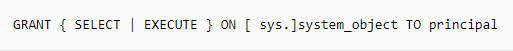
\includegraphics[width=17.5cm]{./Imagenes/3} 
\end{center}

Argumentos \\ \\
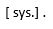
\includegraphics[width=1.5cm]{./Imagenes/sysc} \\ 
Solo se requiere el calificador sys para hacer referencia a vistas de catálogo y vistas de administración dinámica.\\ \\
system\_object\\
Especifica el objeto en el que se va a conceder el permiso.\\
Especifica la entidad de seguridad para la que se concede el permiso.\\
Se asignan privilegios de sistema a un usuario mediante la instrucción "grant":\\ \\
Sintaxis básica:\\ \\
grant PERMISODESISTEMA\\
to USUARIO;\\ \\
Oracle permite conceder múltiples privilegios a múltiples usuarios en una misma sentencia, debemos separarlos por comas.\\ \\
En el siguiente ejemplo se concede el permiso para crear sesión a los usuarios "juan" y "ana": \\
grant create sesion to juan, ana;\\ \\
En el siguiente ejemplo se conceden los permisos para crear tablas y vistas al usuario "ana":\\
grant create table, \\
create view
to ana;\\ \\
En el siguiente ejemplo se conceden 2 permisos a 2 usuarios en una sola sentencia:\\
grant create trigger,\\
create procedure to juan, ana;\\ \\
Consultando el diccionario "dba\_sys\_privs" encontramos los privilegios concedidos a los distintos usuarios; y consultando "user\_sys\_privs" obtendremos la misma información pero únicamente del usuario actual.

